\documentclass[a4paper,12pt]{article}
\usepackage[fontset=none]{ctex}
\usepackage{geometry}
\usepackage{graphicx}
\usepackage{amsmath}
\usepackage{enumitem}
\usepackage{setspace}
\usepackage{fontspec}
\usepackage{booktabs}
\usepackage{caption}
\usepackage{array}
\usepackage{multirow}

% 字体设置（与 docx 模板一致）
\setCJKmainfont{Songti SC}          % 宋体 - 正文默认
\setCJKsansfont{Heiti SC}            % 黑体 - 一级标题
\setCJKmonofont[AutoFakeBold]{STFangsong}          % 仿宋 - 注意事项
\setmainfont{Times New Roman}        % 英文默认

% 页面设置
\geometry{left=2.5cm, right=2.5cm, top=2.5cm, bottom=2.5cm}

% 去掉页码
\pagestyle{empty}

\begin{document}

% ========== 封面 ==========
\begin{center}
    \vspace*{2cm}
    {\fontsize{36pt}{43pt}\selectfont \textbf{物理实验报告}}
    \vspace{3cm}
\end{center}

\begin{center}
    \fontsize{16pt}{24pt}\selectfont
    \textbf{实验名称：弗兰克-赫兹实验\quad} \\[0.5em]
    \textbf{实验桌号：\underline{\quad\quad\quad}} \\[0.5em]
    \textbf{指导教师：\_\_\_\_\_\_\_\_\_\_\_\_\_\_\_\_\_\_\_\_\_\_\_\_\_}
\end{center}

\vspace{2cm}

\begin{center}
    \fontsize{14pt}{28pt}\selectfont
    \textbf{周次：\_\_\_\_\_\_\_\_} \\
    \textbf{姓名：\_\_\_\_\_\_\_\_} \\
    \textbf{学号：\_\_\_\_\_\_\_\_} \\[0.5em]
    \textbf{实验日期: \_\_\_\_年\_\_\_\_月\_\_\_\_日\quad 星期\_\_\_上/下午}
\end{center}

\vspace{1.5cm}

\begin{center}
    \fontsize{14pt}{20pt}\selectfont
    浙江大学物理实验教学中心
\end{center}

\newpage

% ========== 一、预习报告 ==========
{\CJKfontspec{Heiti SC}\fontsize{16pt}{24pt}\selectfont \textbf{一、预习报告}}

\vspace{0.5cm}
{\fontsize{14pt}{20pt}\selectfont \textbf{1. 实验综述}}

\vspace{0.3cm}

{\fontsize{12pt}{18pt}\selectfont

弗兰克-赫兹实验是近代物理学中验证原子能级量子化的经典实验。1914年弗兰克与赫兹用慢电子轰击汞蒸气，测定了汞原子的第一激发电位，有力证明了原子内部存在分立的定态能级，为玻尔原子理论提供了直接实验证据，两人因此获得1925年诺贝尔物理学奖。

实验原理：在充氩弗兰克-赫兹管中，阴极$K$发射的热电子经加速电压$U_{G_2K}$加速后与氩原子碰撞。当电子能量小于氩原子第一激发能量时，仅发生弹性碰撞，板流$I_A$随$U_{G_2K}$增加而增大；当$U_{G_2K}$达到第一激发电势$U_0$时，电子与氩原子发生\textbf{非弹性碰撞}，将能量转移给氩原子使其跃迁至激发态，电子因失去能量无法克服拒斥电压$U_{G_2A}$到达板极，板流$I_A$下降。随$U_{G_2K}$继续增大，板流呈现周期性起伏，相邻峰（谷）值间的电势差即为氩原子第一激发电势，公认值约为$11.61$\,V。

实验装置为THQFH-2A弗兰克-赫兹实验仪，包括弗兰克-赫兹管（充氩四极管）、电源、微电流测量仪和示波器，通过自动扫描或手动逐点测量$I_A$--$U_{G_2K}$曲线，用逐差法求取第一激发电势。

}

\vspace{0.5cm}

{\fontsize{14pt}{20pt}\selectfont \textbf{2. 实验重点}}

\vspace{0.3cm}

{\fontsize{12pt}{18pt}\selectfont

理解原子能级量子化的物理图像及电子与原子碰撞激发的基本方法；掌握弗兰克-赫兹管各电极电压（灯丝电压$U_{F_1F_2}$、栅极电压$U_{G_1K}$、加速电压$U_{G_2K}$、拒斥电压$U_{G_2A}$）的作用及对$I_A$--$U_{G_2K}$曲线的影响；学会用逐差法从峰值电压数据中计算氩原子第一激发电势$U_0$。

}

\vspace{0.5cm}

{\fontsize{14pt}{20pt}\selectfont \textbf{3. 实验难点}}

\vspace{0.3cm}

{\fontsize{12pt}{18pt}\selectfont

合理选择灯丝电压$U_{F_1F_2}$、栅极电压$U_{G_1K}$及拒斥电压$U_{G_2A}$的参数组合，使$I_A$--$U_{G_2K}$曲线峰谷分明且不饱和；手动测量时在峰谷附近需加密测量点以准确定位极值；理解接触电势差导致第一个峰位偏移但不影响相邻峰间距的原因；正确运用逐差法处理数据并分析实验误差。

}

\newpage

% ========== 二、原始数据 ==========
{\CJKfontspec{Heiti SC}\fontsize{16pt}{24pt}\selectfont \textbf{二、原始数据}}

\vspace{0.3cm}
{\fontsize{12pt}{18pt}\selectfont （将有学生和老师签名的"自备数据记录草稿纸"的扫描或手机拍摄图粘贴在下方）}

\vspace{0.5cm}

% 在此粘贴原始数据签名照片:
% \begin{center}
% \includegraphics[width=0.85\textwidth]{原始数据照片.png}
% \end{center}

{\fontsize{12pt}{18pt}\selectfont \textbf{实验仪器参数（实验时记录）：}}

\vspace{0.3cm}

{\fontsize{11pt}{16pt}\selectfont
\begin{tabular}{ll}
    灯丝电压 $U_{F_1F_2}$ = & \_\_\_\_\_\_ V \\[0.5em]
    栅极电压 $U_{G_1K}$ = & \_\_\_\_\_\_ V \\[0.5em]
    拒斥电压 $U_{G_2A}$ = & \_\_\_\_\_\_ V \\[0.5em]
    微电流量程 = & $\times 10^{-9}$\,A \\
\end{tabular}
}

\vspace{0.5cm}

{\fontsize{12pt}{18pt}\selectfont \textbf{表1：自动测量 $I_A$--$U_{G_2K}$ 曲线峰值数据}}

\vspace{0.3cm}

{\fontsize{10.5pt}{15pt}\selectfont
\begin{tabular}{c|ccccccc}
    \toprule
    峰值序号 $n$ & 1 & 2 & 3 & 4 & 5 & 6 & 7 \\
    \midrule
    $U_{G_2K}$（V）第1次 & & & & & & & \\[0.3em]
    $U_{G_2K}$（V）第2次 & & & & & & & \\[0.3em]
    $U_{G_2K}$（V）第3次 & & & & & & & \\[0.3em]
    $U_{G_2K}$（V）第4次 & & & & & & & \\[0.3em]
    $U_{G_2K}$（V）第5次 & & & & & & & \\[0.3em]
    \bottomrule
\end{tabular}
}

\vspace{0.8cm}

{\fontsize{12pt}{18pt}\selectfont \textbf{表2：手动测量 $I_A$--$U_{G_2K}$ 数据}}

\vspace{0.3cm}

{\fontsize{10pt}{14pt}\selectfont
仪器参数：$U_{F_1F_2}$ = \_\_\_\_ V，$U_{G_1K}$ = \_\_\_\_ V，$U_{G_2A}$ = \_\_\_\_ V

\vspace{0.2cm}

\begin{tabular}{c|w{r}{0.72cm} w{r}{0.72cm} w{r}{0.72cm} w{r}{0.72cm} w{r}{0.72cm} w{r}{0.72cm} w{r}{0.72cm} w{r}{0.72cm} w{r}{0.72cm} w{r}{0.72cm}}
    \toprule
    $U_{G_2K}$（V） & 0.5 & 1.0 & 1.5 & 2.0 & 2.5 & 3.0 & 3.5 & 4.0 & 4.5 & 5.0 \\
    \midrule
    $I_A$（nA） & & & & & & & & & & \\
    \bottomrule
\end{tabular}

\vspace{0.1cm}
\begin{center}
    $\cdots\cdots$（按0.5\,V步进继续记录至100\,V）
\end{center}
}

\newpage

% ========== 三、结果与分析 ==========
{\CJKfontspec{Heiti SC}\fontsize{16pt}{24pt}\selectfont \textbf{三、结果与分析}}

\vspace{0.5cm}

{\fontsize{14pt}{20pt}\selectfont \textbf{1. 数据处理与结果}}

\vspace{0.3cm}

{\fontsize{12pt}{18pt}\selectfont

\textbf{（1）$I_A$--$U_{G_2K}$ 曲线}

根据手动测量数据，绘制$I_A$--$U_{G_2K}$曲线，曲线应呈现明显的周期性峰谷结构。

% 在此插入 IA-UG2K 曲线图
% \begin{center}
% 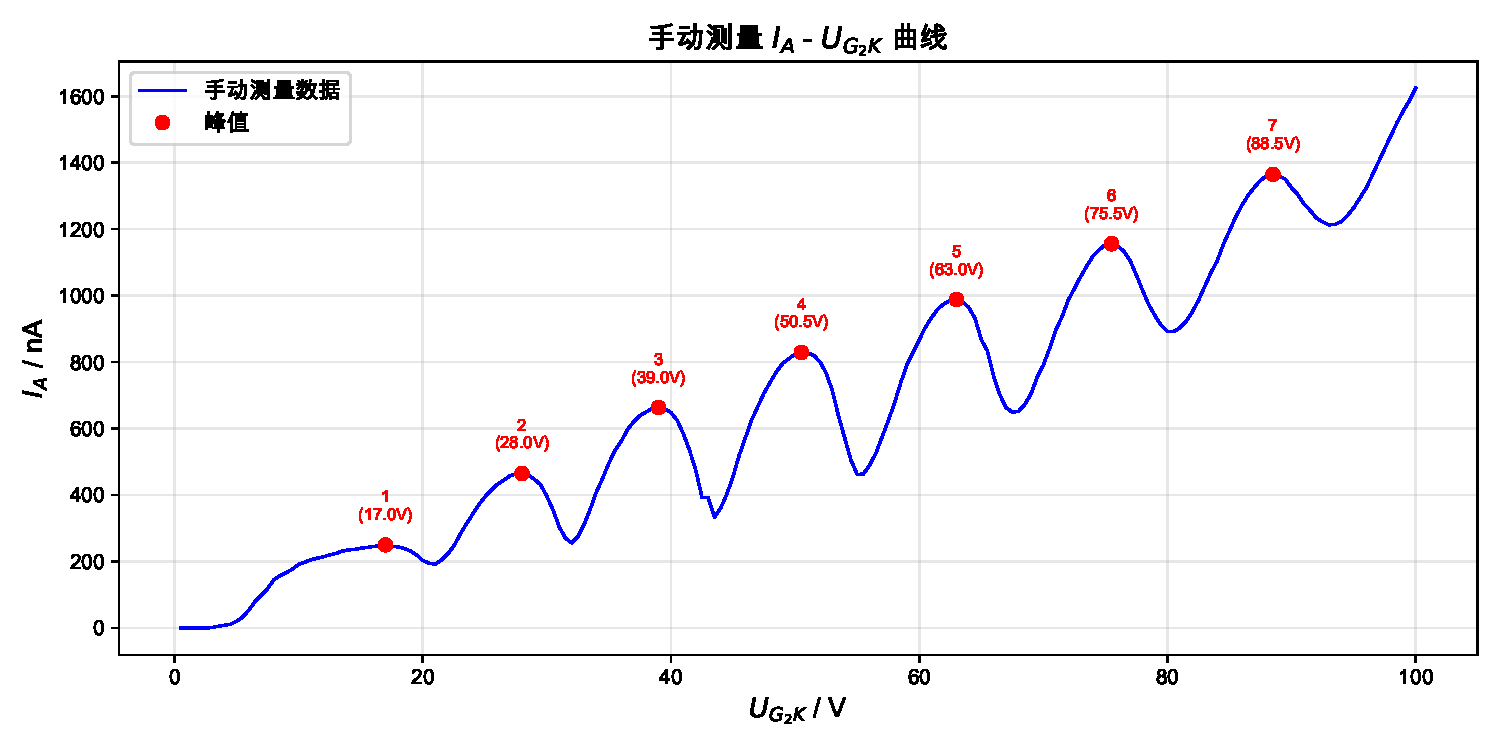
\includegraphics[width=0.9\textwidth]{IA_UG2K_manual.pdf}
% \end{center}

\vspace{0.5cm}

\textbf{（2）用逐差法计算氩原子第一激发电势}

从$I_A$--$U_{G_2K}$曲线中读取各峰值对应的加速电压$U_{G_2K}$，记为$U_1, U_2, \ldots, U_7$。

采用\textbf{逐差法}：将7个峰分为两组，计算
\[
    \Delta U_i = U_{i+4} - U_i, \quad i = 1, 2, 3
\]
每个$\Delta U_i$对应4个峰间距，故单个间距为
\[
    U_{0,i} = \frac{\Delta U_i}{4}
\]
取平均值：
\[
    U_0 = \frac{1}{3}\sum_{i=1}^{3} U_{0,i}
\]

\textbf{（a）自动测量（5次平均）}：

\vspace{0.2cm}

\begin{tabular}{c|ccccccc}
    \toprule
    峰值序号 $n$ & 1 & 2 & 3 & 4 & 5 & 6 & 7 \\
    \midrule
    $\overline{U}_{G_2K}$（V） & & & & & & & \\
    \bottomrule
\end{tabular}

\vspace{0.3cm}

\begin{align}
    \Delta U_1 &= U_5 - U_1 = \text{\_\_\_\_}\text{\,V}, \quad U_{0,1} = \Delta U_1 / 4 = \text{\_\_\_\_}\text{\,V} \notag \\
    \Delta U_2 &= U_6 - U_2 = \text{\_\_\_\_}\text{\,V}, \quad U_{0,2} = \Delta U_2 / 4 = \text{\_\_\_\_}\text{\,V} \notag \\
    \Delta U_3 &= U_7 - U_3 = \text{\_\_\_\_}\text{\,V}, \quad U_{0,3} = \Delta U_3 / 4 = \text{\_\_\_\_}\text{\,V} \notag
\end{align}

\[
    U_0^{(\text{auto})} = \frac{U_{0,1} + U_{0,2} + U_{0,3}}{3} = \text{\_\_\_\_}\text{\,V}
\]

\textbf{（b）手动测量}：

\vspace{0.2cm}

\begin{tabular}{c|ccccccc}
    \toprule
    峰值序号 $n$ & 1 & 2 & 3 & 4 & 5 & 6 & 7 \\
    \midrule
    $U_{G_2K}$（V） & & & & & & & \\
    \bottomrule
\end{tabular}

\vspace{0.3cm}

\begin{align}
    \Delta U_1 &= U_5 - U_1 = \text{\_\_\_\_}\text{\,V}, \quad U_{0,1} = \Delta U_1 / 4 = \text{\_\_\_\_}\text{\,V} \notag \\
    \Delta U_2 &= U_6 - U_2 = \text{\_\_\_\_}\text{\,V}, \quad U_{0,2} = \Delta U_2 / 4 = \text{\_\_\_\_}\text{\,V} \notag \\
    \Delta U_3 &= U_7 - U_3 = \text{\_\_\_\_}\text{\,V}, \quad U_{0,3} = \Delta U_3 / 4 = \text{\_\_\_\_}\text{\,V} \notag
\end{align}

\[
    U_0^{(\text{manual})} = \frac{U_{0,1} + U_{0,2} + U_{0,3}}{3} = \text{\_\_\_\_}\text{\,V}
\]

}

\vspace{0.5cm}

{\fontsize{14pt}{20pt}\selectfont \textbf{2. 误差分析}}

\vspace{0.3cm}

{\fontsize{12pt}{18pt}\selectfont

氩原子第一激发电势公认值为$U_{0,\text{ref}} = 11.61$\,V。

相对误差：
\[
    E_r = \frac{|U_0 - U_{0,\text{ref}}|}{U_{0,\text{ref}}} \times 100\%
\]

\textbf{不确定度分析}（以自动测量5次数据为例）：

对5次自动测量分别用逐差法求得$U_0$：$U_{0,1}', U_{0,2}', \ldots, U_{0,5}'$。

A类标准不确定度：
\[
    u_A = \sqrt{\frac{\displaystyle\sum_{i=1}^{n}(U_{0,i}' - \bar{U}_0)^2}{n(n-1)}}
\]

取置信概率$P = 0.95$，自由度$\nu = n - 1 = 4$，查$t$分布表得$t_{0.95}(4) = 2.776$，扩展不确定度为：
\[
    U = t_{0.95}(4) \cdot u_A
\]

最终结果表示为：
\[
    U_0 = (\bar{U}_0 \pm U)\text{\,V}, \quad P = 0.95
\]

\vspace{0.3cm}

实验中的主要误差来源：

（1）\textbf{接触电势差}：阴极、板极和连接导线材料不同产生的接触电位差，使$I_A$--$U_{G_2K}$曲线沿电压轴整体偏移，导致第一个峰值位置偏离理论值，但不影响相邻峰间距。

（2）\textbf{热电子能量分布}：阴极发射的热电子具有麦克斯韦分布，使峰谷位置具有一定展宽，导致读取极值电压时存在不确定度。

（3）\textbf{亚稳态效应}：氩原子基态与第一激发态之间存在两个亚稳态（电势差分别为$11.55$\,V和$11.72$\,V），实验测得的第一激发电势实际对应基态到亚稳态的跃迁，介于$11.55$\,V$\sim$$11.72$\,V之间。

（4）\textbf{仪器读数误差}：手动测量时$U_{G_2K}$步进为0.5\,V，峰值定位精度受限。

}

\vspace{0.5cm}

{\fontsize{14pt}{20pt}\selectfont \textbf{3. 实验探讨}}

\vspace{0.3cm}

{\fontsize{12pt}{18pt}\selectfont

（在此填写实验小结，不超过100字）

}

\newpage

% ========== 四、思考题 ==========
{\CJKfontspec{Heiti SC}\fontsize{16pt}{24pt}\selectfont \textbf{四、思考题}}

\vspace{0.5cm}

{\fontsize{12pt}{18pt}\selectfont

\textbf{1. 原子第一激发态的物理意义}

根据玻尔原子理论，原子只能处于一系列分立的定态能级$E_1 < E_2 < E_3 < \cdots$，其中$E_1$为基态。\textbf{第一激发态}是指能量为$E_2$的最低激发态，原子从基态跃迁到第一激发态所需的最小能量$\Delta E = E_2 - E_1$称为\textbf{临界能量}，对应的电势$U_0 = \Delta E / e$称为\textbf{第一激发电势}。

第一激发态的物理意义在于：它是原子被外界激发时最容易达到的激发态，也是验证原子能级分立性的最直接证据。在弗兰克-赫兹实验中，当电子动能恰好达到$eU_0$时，电子与原子发生非弹性碰撞，原子从基态跃迁到第一激发态，$I_A$--$U_{G_2K}$曲线出现周期性峰谷结构，其间距即为第一激发电势。对于氩原子，基态与第一激发态之间还存在两个亚稳态（电势差分别为$11.55$\,V和$11.72$\,V），实验中测得的$U_0 \approx 11.61$\,V实际对应基态到亚稳态的跃迁。

\vspace{0.5cm}

\textbf{2. 温度对$I$--$U$曲线的影响}

温度对$I_A$--$U_{G_2K}$曲线的影响主要体现在以下方面：

（1）\textbf{气体原子热运动加剧}：温度升高时，管内氩原子的热运动速度增大，电子与氩原子碰撞的相对速度发生变化，使得非弹性碰撞发生的加速电压$U_{G_2K}$产生展宽。宏观上表现为$I_A$--$U_{G_2K}$曲线的峰和谷变得更加平坦、峰谷差减小，极值位置的读取精度下降。

（2）\textbf{气体密度变化}：温度升高导致氩气密度降低（在密封管中压强升高但平均自由程变化），电子在加速过程中与氩原子碰撞的概率改变，影响非弹性碰撞的效率。

（3）\textbf{阴极热电子发射增强}：温度升高使灯丝发射的热电子数增多、初始能量分布更宽（麦克斯韦分布展宽），导致曲线整体上移，峰谷边界更模糊。

（4）\textbf{对汞管的影响尤为显著}：若使用充汞弗兰克-赫兹管，温度直接决定管内汞蒸气压，温度过低则汞蒸气稀薄、碰撞概率低、峰谷不明显；温度过高则汞蒸气过浓、电子平均自由程过短、无法积累足够能量到达板极，曲线峰值急剧下降。因此充汞管需在$150\sim200\,^\circ$C范围内精确控温。

}

\vfill

% ========== 注意事项 ==========
\noindent\rule{\textwidth}{0.4pt}

{\CJKfontspec[AutoFakeBold]{STFangsong}\fontsize{12pt}{18pt}\selectfont
\textbf{注意事项：}
\begin{enumerate}[label=\arabic*., leftmargin=2em, nosep]
    \item 用PDF格式上传"实验报告"，文件名：学生姓名+学号+实验名称+周次。
    \item "实验报告"必须递交在"学在浙大"的本课程的对应实验项目的"作业"模块内。
    \item "实验报告"成绩必须在"浙江大学物理实验教学中心网站"-"选课系统"内查询。
    \item 教学评价必须在"浙江大学物理实验教学中心网站"-"选课系统"内进行，学生必须进行教学评价，才能看到实验报告成绩，教学评价必须在本次实验结束后3天内进行。
\end{enumerate}
}

\vspace{0.5cm}
\begin{center}
    {\CJKfontspec[AutoFakeBold]{STFangsong}\fontsize{12pt}{18pt}\selectfont \textbf{浙江大学物理实验教学中心制}}
\end{center}

\end{document}
